\documentclass{beamer}
\usetheme{Madrid}

\usepackage{amsmath, amssymb, amsthm}
\usepackage{graphicx}
\usepackage{listings}
\usepackage{gensymb}
\usepackage[utf8]{inputenc}
\usepackage{hyperref}
\usepackage{gvv}
\newcommand{\mySolution}{\noindent \textbf{Solution: }}
\begin{document}

\title{matgeo-9.3.18}
\author{EE22BTECH11009 - Mokshith Kumar$^{}$
}
\frame{\titlepage}
\begin{frame}
\frametitle{Question}
Using integration, find the area of the smaller region enclosed by the curve $4x^2 + 4y^2 = 9$ and the line $2x + 2y = 3$.\hfill{9.3.18}
\end{frame}
\begin{frame}
\frametitle{\mySolution}
The given circle can be expressed as conics with parameters,
\begin{align}
    V=\myvec{4 & 0\\0 & 4}, u=0, f=-9.
\end{align}
The line parameters are:
\begin{align}
    h=\myvec{0\\ \frac{3}{2}}, m=\myvec{1\\-1}.
\end{align}
The points of intersection of the line 
\begin{align}
L: \quad x = h + \kappa m \quad \kappa \in \mathbb{R}
\end{align}
with the conic section 
\begin{align}
    \text{g}\brak{x} = x^{\top}Vx + 2u^{\top}x + f = 0
\end{align}
are given by
\begin{align}
x_i = h + \kappa_i m
\end{align}
where,
\begin{multline}
\kappa_i = \frac{1}{m^{\top}Vm} \left( -m^{\top}(Vh+u) \right) \\
\pm \sqrt{
\left( m^{\top}(Vh+u) \right)^2 - g(h) \cdot (m^{\top}Vm)
}
\end{multline}
Substituting the parameters in the above equation yields:
\begin{align}
    k=0,\frac{3}{2}.
\end{align}
This gives the points of intersection as:
\begin{align}
    A=\myvec{\frac{3}{2}\\0}, B=\myvec{0\\ \frac{3}{2}}.
\end{align}
From \figref{plot}, the desired area is:
\begin{align}
\int_{0}^{\frac{3}{2}}\frac{\sqrt{9-4x^2}}{2}-\int_{0}^{\frac{3}{2}}\frac{3-2x}{2}=\frac{9}{16}\pi-\frac{9}{8}.
\end{align}
\end{frame}

\begin{frame}{allowframebreaks}
\frametitle{Figure}
\begin{figure}[h!]
   \centering
   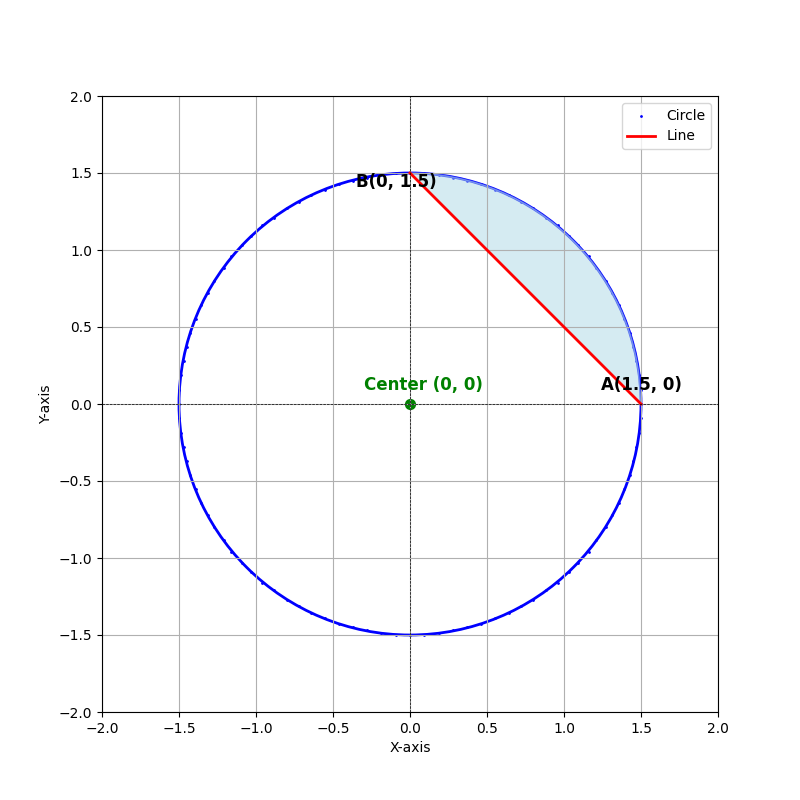
\includegraphics[width=0.7\linewidth]{figs/plot.png}
   \caption{ }
   \label{plot}
\end{figure}\\
\end{frame}
\begin{frame}{allowframebreaks}
\frametitle{Table}
\begin{table}[h]
    \centering
    \begin{tabular}{|c|c|}
        \hline
        Point & Coordinates\\
        \hline
        $A$ & \myvec{0\\6}\\
        \hline
        $B$ & \myvec{8\\0}\\
        \hline
        $C$ & \myvec{0\\0}\\
        \hline
\end{tabular}

    \caption{Parameters used}
    \label{}
\end{table}
\end{frame}
\end{document}